\subsection{Kho hội nghị 2020--2026 và tìm kiếm ngoài snapshot}
Pipeline mở rộng thu thập metadata ICML, NeurIPS, ICLR, AAAI, EMNLP, NAACL, ACL và CVPR. ICML dùng volume PMLR; ICLR/NeurIPS dùng JSON của chương trình chính thức; ACL-family dùng XML ở commit cố định của ACL Anthology, gồm Findings theo đúng volume hội nghị; CVPR dùng CVF Open Access. OpenAlex bổ sung metadata qua source ID và cursor đến hết kết quả; AAAI hiện dùng nguồn này. URL từng lần fetch, trạng thái nguồn và SHA-256 của JSONL nằm trong manifest.

Collector có gzip cache theo URL, retry có giới hạn và ba worker. Khi chạy lại, dữ liệu đã tải được tái sử dụng. Bộ đọc nhận dạng khác biệt giữa program cũ/mới, loại session cha, loại workshop trong program và nối các trang CVPR theo ngày. Chuẩn hóa tiêu đề được dùng để khử trùng trong từng hội nghị/năm; giữ OpenAlex ID nếu có để nối references. Alias chính thức được lưu cùng bản ghi. Phép join này có thể bỏ sót biến thể tiêu đề hoặc hợp nhất nhầm tên giống nhau; chưa có fuzzy entity resolution.

Snapshot mở rộng chứa \CatalogCount{} bản ghi, trong đó \CatalogAbstractPercent\% có abstract. Đây là số metadata thu được từ các nguồn đã hoàn tất, không phải tổng số paper được chấp nhận đã kiểm chứng độc lập. Phạm vi có thể gồm Findings, short paper hoặc track khác được nguồn công bố. EMNLP 2026 và NAACL 2020/2023/2026 chưa có bản ghi từ các adapter tại thời điểm thu thập; ô 0 không được diễn giải thành hội nghị không tồn tại. Không tải hàng loạt PDF.
\fig{conference_coverage.pdf}{1}{Coverage sau khử trùng của snapshot mở rộng. Các số là bản ghi thu thập được; không trộn vào corpus 3.595 paper của thí nghiệm gốc.}
\FloatBarrier

Kho hội nghị dùng inverted index FTS5 trên đĩa \cite{fts5}, với trọng số BM25 cho title/abstract/authors/conference lần lượt là 8/2/2/1. Query được tách thành tối đa 32 token, nối OR, kết hợp bộ lọc hội nghị/năm và phân trang. Không đưa toàn bộ hơn một trăm nghìn paper vào NetworkX hoặc ma trận recommendation lúc startup. API truy hồi và giao diện hiển thị rõ backend này khác ranking trong mining workspace.
\begin{figure}[H]\centering
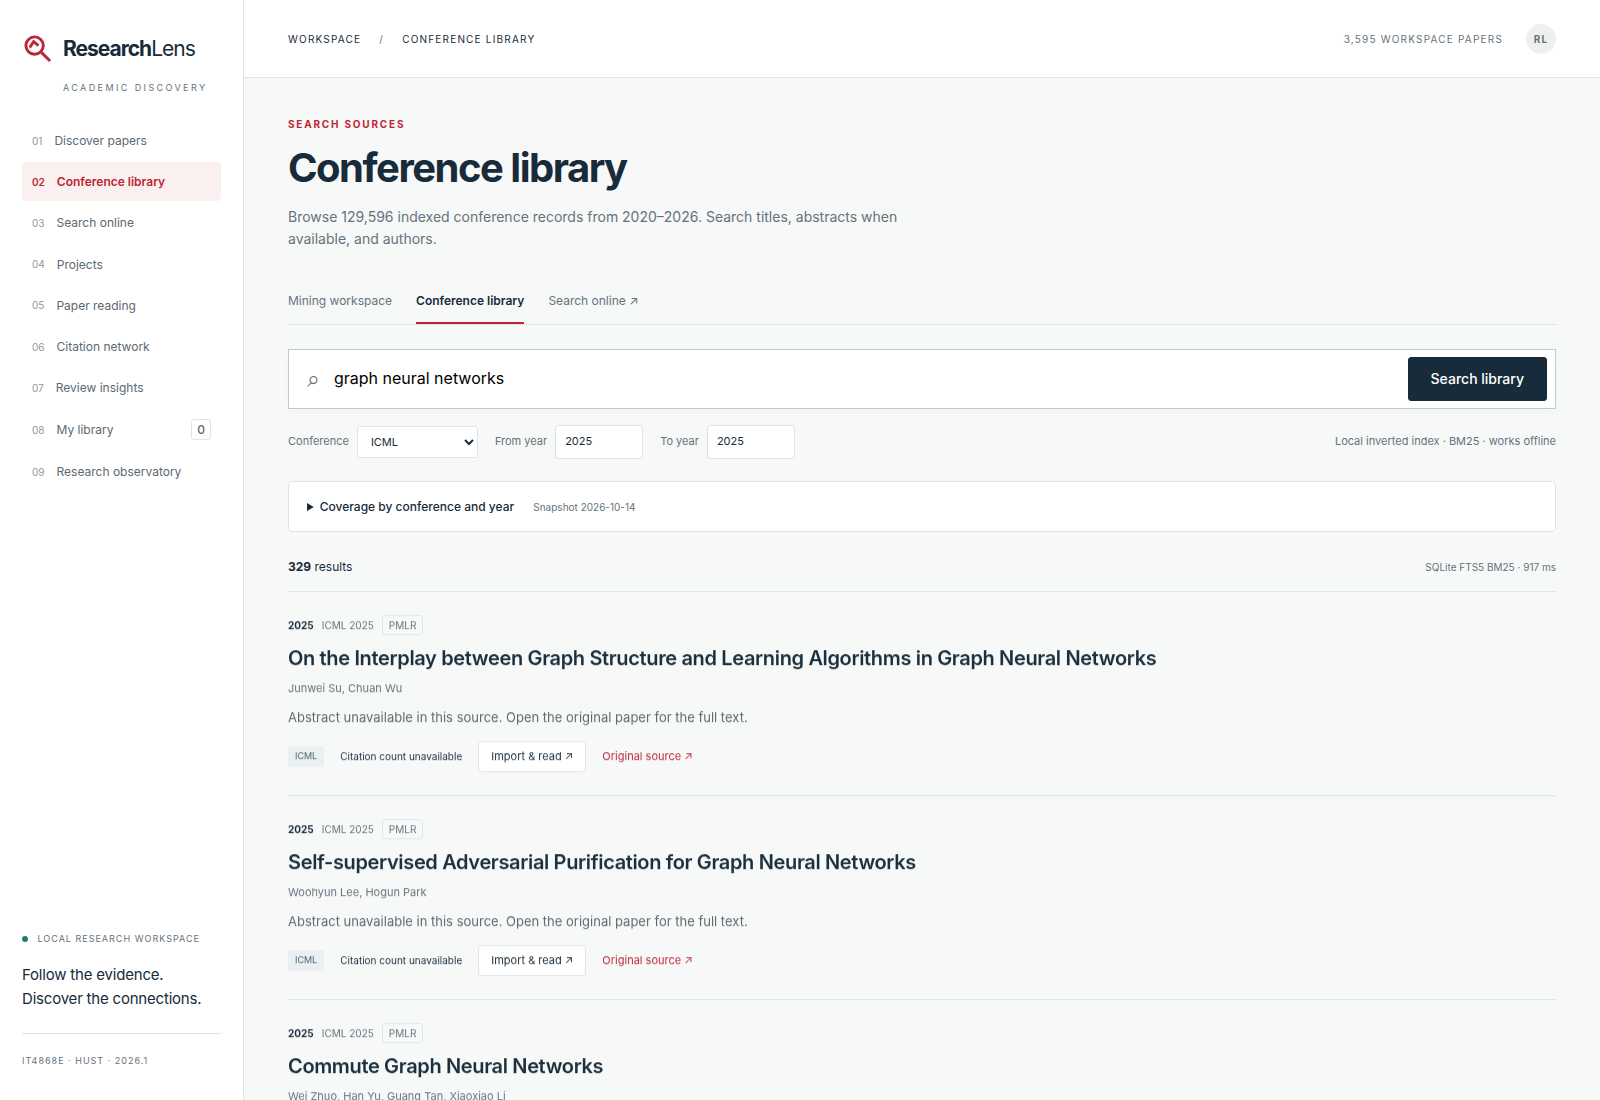
\includegraphics[width=\textwidth]{conferences.png}
\caption{Tìm kiếm thật trên kho hội nghị: query graph neural networks, ICML 2025. Abstract hoặc citation count thiếu được ghi rõ; không sinh nội dung thay thế.}
\end{figure}

Search online gửi query và lọc năm đến OpenAlex \cite{openalexsearch}, cache metadata năm phút, giới hạn 128 cache entries. API key tùy chọn nằm ở server; lỗi quota hoặc metadata sai kiểu được trả thành lỗi dịch vụ có kiểm soát. Kết quả chưa tự gia nhập graph. Nút \textit{Import \& read} lấy lại metadata từ provider theo ID, khử trùng DOI/tiêu đề và lưu bền. Với record chính thức, hệ thống thử tìm exact match để bổ sung abstract/references; nếu không có, giao diện thông báo giới hạn enrichment.

Import tạo một mining engine mới trước khi ghi/swap; lock tuần tự hóa các import trong một process. Mapping alias được áp dụng lên references cả khi import và khi khởi động lại. Nhờ vậy paper có OpenAlex ID khác với ID chính thức vẫn nối đúng cạnh citation. Corpus import dùng chung trong instance; Project, notes và thư viện vẫn riêng theo profile trình duyệt. Chưa hỗ trợ đồng bộ engine giữa nhiều worker. Apache Solr tùy chọn tiếp tục index snapshot gốc, không tự nhận paper import.
\begin{figure}[H]\centering
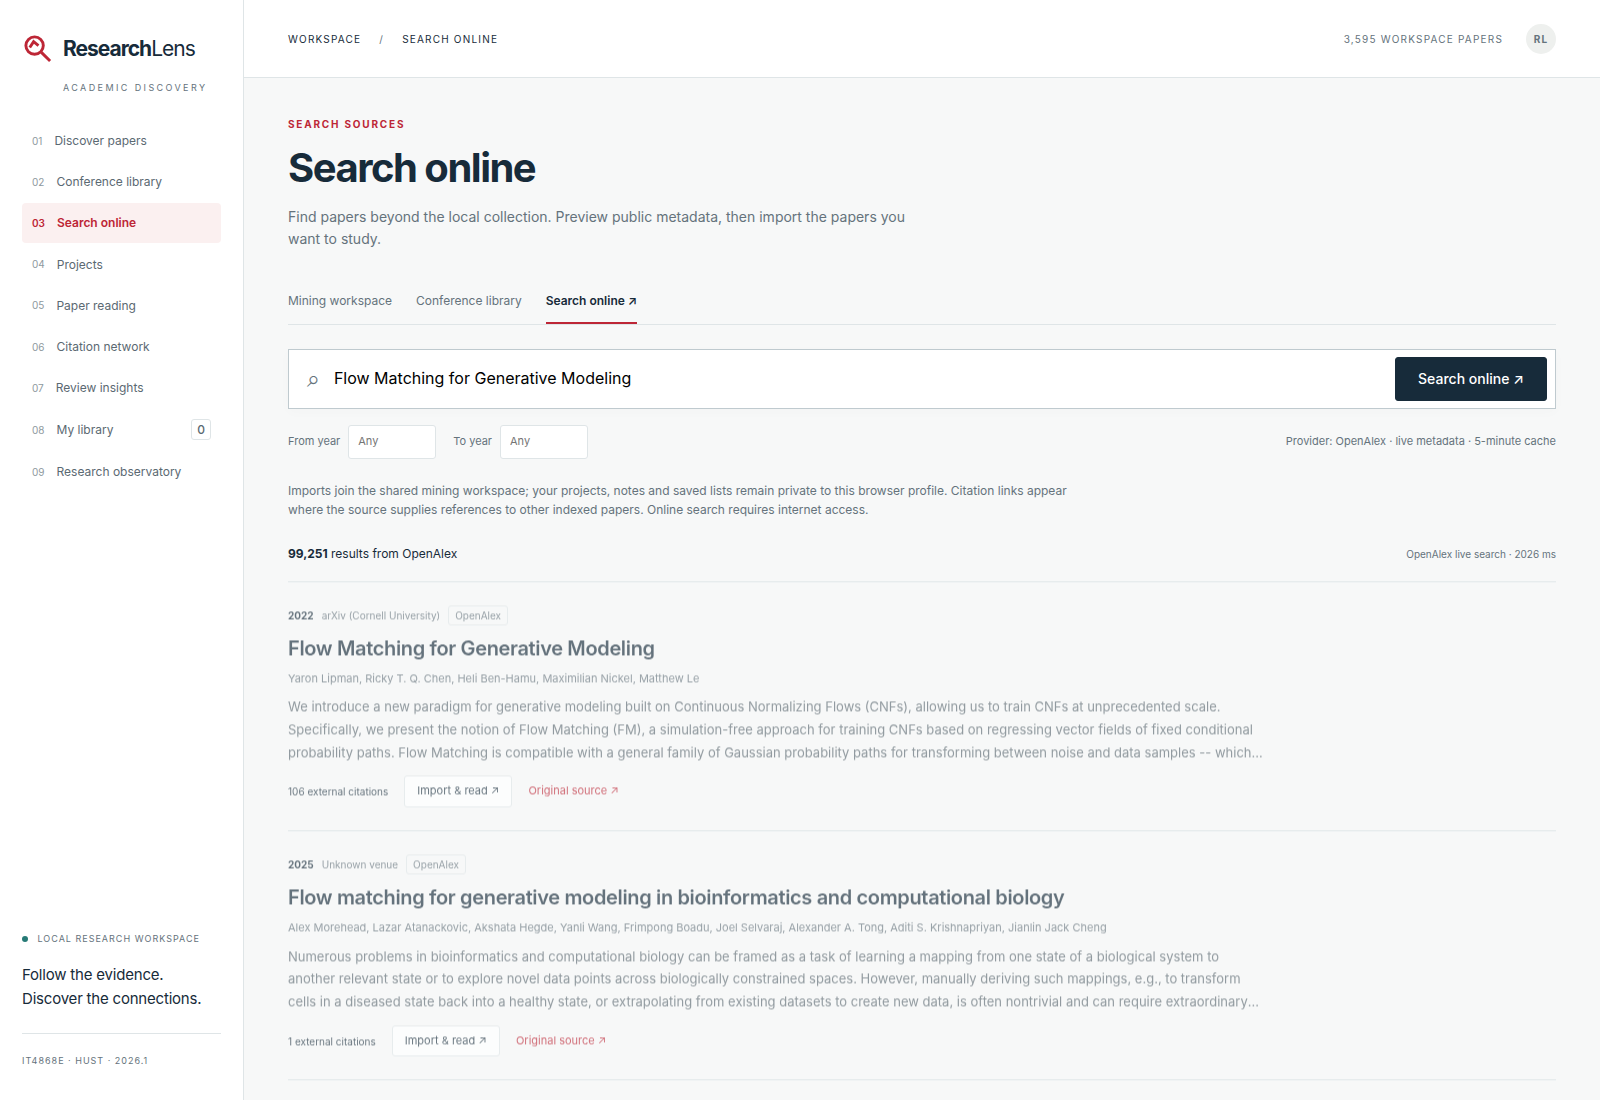
\includegraphics[width=\textwidth]{online_search.png}
\caption{Search online với metadata OpenAlex thật. Paper có thể import vào reader, thêm vào Project và tham gia citation graph nếu có reference khớp. Không tạo cạnh khi nguồn không cung cấp bằng chứng.}
\end{figure}

\subsection{Đo hiệu năng riêng cho kho hội nghị}
Script \texttt{scripts/evaluate\_catalog.py} dựng index mới và đo 20 query chủ đề cố định qua năm vòng, tổng cộng 100 lần đo. Mỗi query được warm một lần; các vòng xen kẽ có/không lọc hội nghị. Phạm vi gồm đếm kết quả, BM25, top-20 và giải mã JSON; không gồm HTTP, browser hoặc mạng. Trên môi trường lưu trong artifact, dựng index mất \CatalogBuildSeconds{} giây, database chiếm \CatalogIndexMiB{} MiB; latency p50 là \CatalogLatencyMedian{} ms, p95 là \CatalogLatencyTail{} ms.

Đây là phép đo mô tả trên một máy, single process, không phải load test hay kết luận về relevance. Tất cả 100 quan sát nằm trong \texttt{artifacts/catalog\_results.json}. Chưa có nhãn relevance cho kho mới nên không gán nDCG của SciFact hoặc reference recovery cũ cho 129 nghìn record này. Import thay đổi thống kê workspace đang chạy, nhưng không thay JSONL hay số đo benchmark gốc.
